%%%%%%%%%%%%%%%%%%%%%%%%%%%%%%%%%%%%%%%%%
% Demostración de la NP-Completitud del 
% problema de CLIQUE
% Complejidad Computacional
% Universidad de La Laguna
%
% Alejandro León Fernández
% Javier Esteban Pérez Rivas
% Sara Revilla Báez
%%%%%%%%%%%%%%%%%%%%%%%%%%%%%%%%%%%%%%%%%

%----------------------------------------------------------------------------------------
%	PACKAGES AND THEMES
%----------------------------------------------------------------------------------------

\documentclass{beamer}

\mode<presentation> {
\usetheme{Madrid}
}

\usepackage{graphicx} % Allows including images
\usepackage{booktabs} % Allows the use of \toprule, \midrule and \bottomrule in tables
\usepackage{amsmath}

% Spanish
\usepackage[spanish]{babel}
\usepackage[utf8]{inputenc}

%----------------------------------------------------------------------------------------
%	TITLE PAGE
%----------------------------------------------------------------------------------------

\title[NP-Completitud de CLIQUE]{Demostración de NP-Completitud del problema de CLIQUE}

\author[A.L.F., J.P.R., S.R.B.]{
    Alejandro León Fernández \\
    Javier Esteban Pérez Rivas \\
    Sara Revilla Báez
}

\institute[ULL]{Universidad de La Laguna}
\date{16 de enero de 2019}

\begin{document}

\begin{frame}
    \titlepage % Print the title page as the first slide
\end{frame}

\begin{frame}
    \frametitle{Índice}
    \tableofcontents
\end{frame}

%----------------------------------------------------------------------------------------
%	PRESENTATION SLIDES
%----------------------------------------------------------------------------------------

%------------------------------------------------
\section{Introducción}
%------------------------------------------------

\subsection{¿Qué es un clique?}

\begin{frame}
\frametitle{¿Qué es un clique?}
    \begin{block}{Definición}
    Un clique es un subconjunto de vértices de un grafo no dirigido, tal que cada par de vértices sea adyacente. Es decir, que su subgrafo inducido es completo.
    \end{block}
    El término se usó por primera vez en un trabajo Luce \& Perry (1949) en referencia a los grupos de personas que se conocen entre todas ellas.
    
    \begin{figure}
    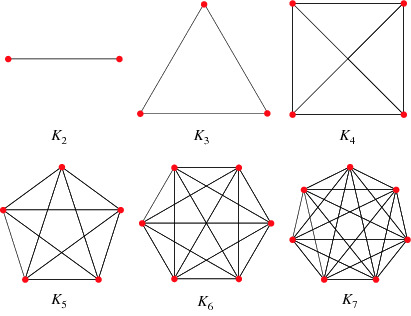
\includegraphics[width=0.5\linewidth]{img/complete_graphs.jpg}
    \end{figure}
\end{frame}

\subsection{Descripción del problema}

\begin{frame}
\frametitle{Descripción del problema}
    \begin{block}{INSTANCIA}
    Se tiene un grafo $G=(V, E)$ y un entero positivo $k$.
    \end{block}
    \begin{block}{PREGUNTA}
    \centering ¿Existe un $k$-clique en $G$? \\
    Es decir, que si existe un conjunto de vertices $V' \subseteq V$ tal que, 
    $$ |V'| \geq k $$
    $$ \forall u, v \in S \implies \exists (u, v) \in E $$
    \end{block}
\end{frame}

%------------------------------------------------
\section{Demostración de NP-completitud}
%------------------------------------------------

\begin{frame}
\frametitle{Demostración de NP-completitud}

    \begin{block}{Definición}
    Para demostrar que el problema de CLIQUE es NP-completo, debemos probar que:
    \begin{enumerate}[I]
        \item CLIQUE está en NP
        \item Existe una transformación de cualquier problema de la clase NP a CLIQUE o, alternativamente, que existe una transformación de un problema NP-completo a CLIQUE
    \end{enumerate}
    \end{block}
    
\end{frame}

%------------------------------------------------
\subsection{CLIQUE está en NP}

\begin{frame}
\frametitle{CLIQUE está en NP}
    \begin{theorem}
    Si encontramos un algoritmo no determinista que decida si para un grafo $G = (V,E)$ existe un clique de tamaño mayor o igual que $k$, entonces podemos afirmar que el problema de CLIQUE $\in$ NP.
    \end{theorem}
    
    \begin{proof}
    Para ello, basta con probar con todos los $V' \subseteq V$ tal que $\vert V' \vert \geq k$ y ver si alguno de ellos es un clique.
    
    Esta comprobación se puede realizar en tiempo polinomial mirando que $(u,v) \in E$ para cada $u, v \in S$, lo cual tiene complejidad $O(n^2)$.
    \end{proof}
\end{frame}

%------------------------------------------------

\begin{frame}{Inciso}

    Existe una secuencia de transformaciones que permiten demostrar que el CLIQUE es reducible al SAT de manera prácticamente trivial (comparándolo con el VC). Sin embargo, vamos a plantear una transformación directa del 3-SAT al CLIQUE.

    \begin{figure}
    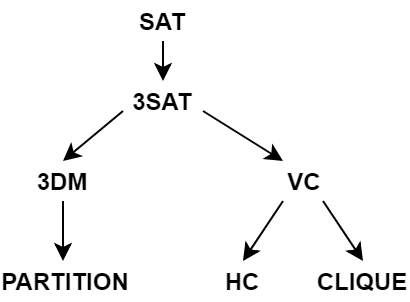
\includegraphics[width=0.5\linewidth]{img/problem-diagram.png}
    \caption{Diagrama de la secuencia de transformaciones de los 6 problemas básicos}
    \end{figure}

    
\end{frame}

%------------------------------------------------

\subsection{Transformación del 3-SAT al CLIQUE}
\begin{frame}
\frametitle{Transformación del 3-SAT al CLIQUE}
    \begin{block}{3-SAT}
    \begin{itemize}
        \item INSTANCIA: Dada una colección $C = \{c_{1}, c_{2}, ..., c_{m}\}$ de cláusulas con un conjunto $X = \{x_{1}, x_{2}, ..., x_{n}\}$ de variables, tal que $\vert c_{i} \vert$ = 3 para $1 \geq \textit{i} \geq m$
        \item PREGUNTA: ¿Existe alguna asignación de verdad para $X$ que satisfaga todas las cláusulas en $C$?
    \end{itemize}
    \end{block}
\end{frame}

%------------------------------------------------

\begin{frame}
\frametitle{Transformación del 3-SAT al CLIQUE (II)}
    \begin{block}{Transformación}
    Dada $\phi$ una instancia de 3-SAT tal como hemos descrito, y cada cláusula $c_{i} = \{z_{i1}, z_{i2}, ..., z_{it}\}$ (con $t = 3$), necesitamos construir una instancia del CLIQUE (un grafo), que sea positiva si y solo si $\phi$ también es positiva.
    \end{block}
\end{frame}


%------------------------------------------------

\begin{frame}
\frametitle{Transformación del 3-SAT al CLIQUE (III)}
    \begin{block}{Grafo}
    Construimos un grafo $G = (V,E)$ de la siguiente forma:
    \begin{enumerate}
        \item En primer lugar añadimos $t$ nodos por cada cláusula. Este paso se hace en tiempo $O(t \cdot m)$ que es $O(m)$ ya que $t = 3$.
        \item Para cada par de nodos $v_{ab},v_{cd}$ en $G$, añadimos la arista $(v_{ab},v_{cd})$ si y solo si:
        \begin{itemize}
            \item $a \neq c$
            \item $z_{ab} \neq \bar{z}_{cd}$
        \end{itemize}
    \end{enumerate}
    \end{block}
    
    $\phi$ es satisfactible si y solo si $G$ tiene un clique de tamaño $k \geq m$.
    
\end{frame}

%------------------------------------------------

\begin{frame}
\frametitle{Transformación del 3-SAT al CLIQUE (IV)}
    \begin{proof}
    Si $\phi$ es satisfactible, elegimos un literal satisfecho de cada cláusula obteniendo $\{z_{1}^{*}, z_{2}^{*}, ..., z_{m}^{*}\}$, siendo $\{v_{1}, v_{2}, ..., v_{m}\}$ los nodos correspondientes en $G$. Dicho conjunto de nodos forma un m-clique, pues estarán conectados ya que:
    \begin{itemize}
        \item Hemos escogido los literales de diferentes cláusulas
        \item No puede haber contradicciones entre los literales escogidos porque $\phi$ es satisfactible
    \end{itemize}
    \end{proof}
\end{frame}

%------------------------------------------------

\begin{frame}
\frametitle{Transformación del 3-SAT al CLIQUE (V)}
    \begin{proof}
    Viceversa, supongamos que $G$ tiene un clique de tamaño $m = k$ o mayor. Sea $\{v_{1}, v_{2}, ..., v_{q}\}$ un clique en $G$ de tamaño $q \geq m$. Entonces los $m$ primeros nodos $\{v_{1}, ..., v_{m}\}$ también forman un clique en $G$.
    \begin{itemize}
        \item Dado que no hay aristas conectando nodos que vengan de la misma cláusula, cada uno de los nodos corresponde a un literal de una cláusula.
        \item Además, no hay nodos que vengan de literales opuestos conectados debido a la construcción realizada
    \end{itemize}
    Así, para satisfacer $\phi$ basta con satisfacer $\{z_{1}, ..., z_{m}\}$ y asignar las variables restantes de forma arbitraria.
    \end{proof}
\end{frame}

%------------------------------------------------

\subsection{Ejemplo}

\begin{frame}{Ejemplo (I)}
Sea $\phi$ una instancia de 3-SAT, con variables $x_{i}$, para $i$ en $1 \leq i \leq 3$, se obtiene el siguiente grafo aplicando la reducción comentada anteriormente. 
\begin{block}{Problema}
$$\phi = (x_{1}\lor \bar{x}_{2} \lor \bar{x}_{3}) \land (\bar{x}_{1} \lor x_{2} \lor x_{3}) \land (x_{1} \lor x_{2} \lor x_{3})$$
\end{block}

\begin{figure}
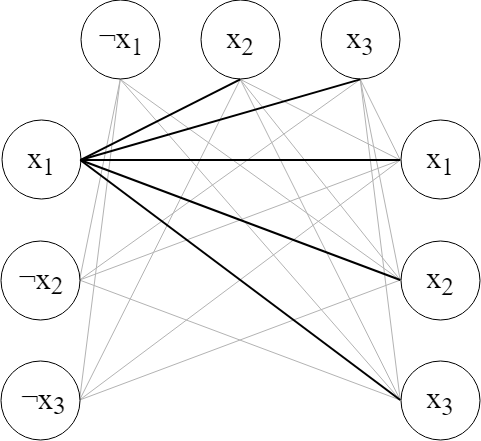
\includegraphics[width=0.4\linewidth]{img/Grafo_Ejemplo_Clique.png}
\caption{Grafo resultante}
\end{figure}
\end{frame}

%------------------------------------------------
\begin{frame}{Ejemplo (II)}
Elegimos una variable, $z_{i}$, dentro de cada cláusula y suponemos que son verdaderas. Cada una se corresponde con un nodo dentro del grafo. $\phi$ se podrá satisfacer si, y solo si, existe un \textbf{clique} para los nodos elegidos. Para este ejemplo, elegiremos $x_{1}$ como variable positiva de la primera cláusula,  $x_{2}$, para la segunda, y $x_{3}$, para la tercera.
\begin{figure}
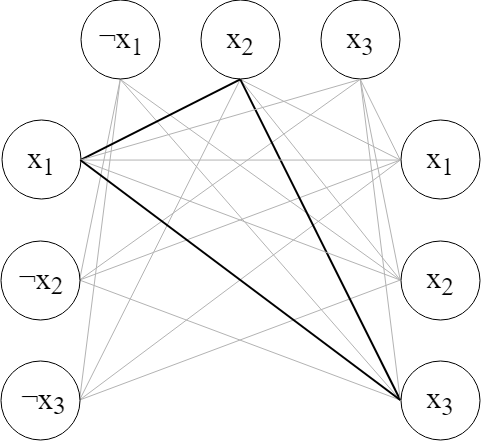
\includegraphics[width=0.4\linewidth]{img/Grafo_Seleccion_Clique.png}
\caption{Clique}
\end{figure}
\end{frame}


%------------------------------------------------
\begin{frame}
\frametitle{Bibliografía}
\footnotesize{
    \begin{thebibliography}{99}
        \bibitem{GareyJohnson}
            Michael Garey, David S. Johnson.
        \newblock {\em Computers and Intractability: A Guide to the Theory of NP-Completeness}.
        \newblock W. H. Freeman and Company, 1979.
        
        \bibitem{Mouatadid}
            Lalla Mouatadid.
        \newblock {\em Introduction to Complexity Theory: CLIQUE is NP-complete}.
        \newblock CSC 373 - Algorithm Design, Analysis, and Complexity, Summer 2014.
    \end{thebibliography}
}
\end{frame}

%------------------------------------------------

\begin{frame}

\centering 
{\Huge{Gracias}}
\vfill
    Alejandro León Fernández \\
    Javier Esteban Pérez Rivas \\
    Sara Revilla Báez

\end{frame}

%----------------------------------------------------------------------------------------

\end{document} 